\chapter{Studiu conectare MPTCP în rețeaua ORO}
\label{sec:oro_arch}

\section{Caracteristicile rețelei 3G/4G ORO}

Reţeaua ORO, prezentată în figura \ref{fig:oro_network}, oferă atât
servicii de date mobile folosind rețeaua celulară, cât şi servicii de
conectare la internet folosind reţele WiFi.  In cazul reţelei 3G/4G,
accesul se face prin echipamentele NodeB, RNC, EPG pentru sesiunile
3G, respectiv eNodeB, MME, EPG pentru sesiunile 4G, iar tot traficul
este filtrat prin echipamentele de tip Firewall, de unde se face
accesul către internet.  Orange Romania oferă si rețele Wi-Fi pentru
accesul la internet, folosindu-se de echipamente de tip Access Point,
iar traficul este agregat central in rețea in WLAN GW.  Clienții
folosesc un APN a primi acces la internet, iar clienții comerciali
folosesc APN-ul net. Pentru aceștia, opțiunile extra din protocolul
TCP precum MPTCP sunt tăiate de către Firewall-uri, așadar pentru
implementarea acestui serviciu de tip 4.5G sunt necesare configurarea
unui APN dedicat si configurarea si realizarea unei configurații
speciale in rețea pentru plasarea Proxy-ului MPTCP.

\begin{figure}[h]
	\centering
	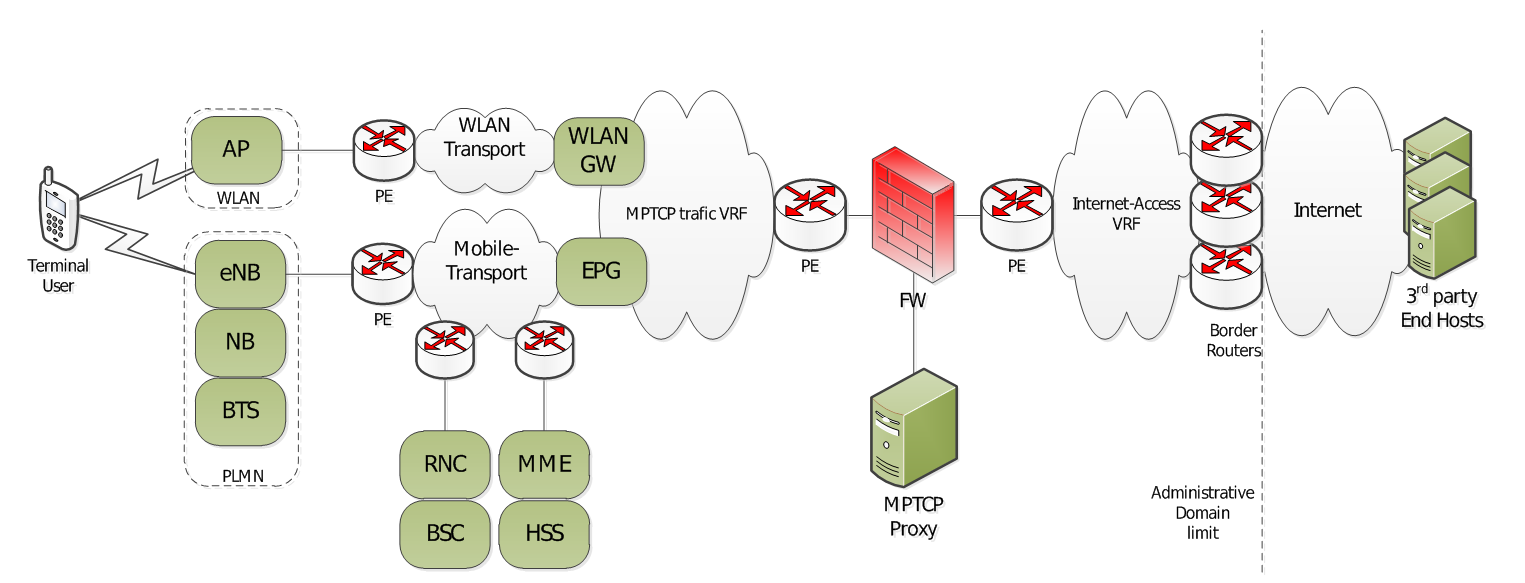
\includegraphics[scale=0.3]{figures/oro/oro_network.png}
	\caption{Structura generală a rețelei de test}
    	\label{fig:oro_network}
\end{figure}


\section{Plasarea proxy-ului MPTCP în rețeaua SGi-LAN}

\begin{figure}[h]
	\centering
	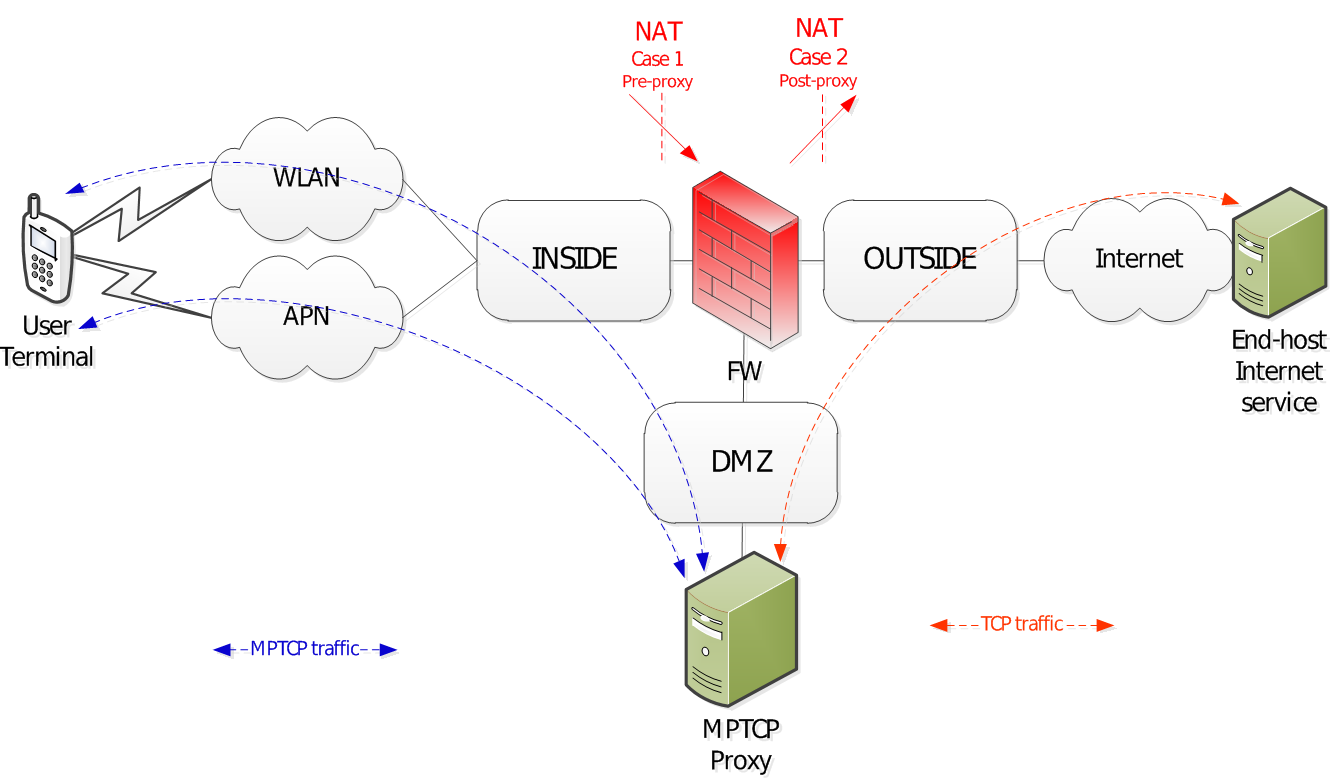
\includegraphics[scale=0.3]{figures/oro/oro_mptcp.png}
	\caption{Plasarea proxy-ului de MPTCP în spatele unui firewall cu trei zone}
    	\label{fig:oro_mptcp}
\end{figure}

Serviciul MPTCP va fi testat utilizând un APN dedicat, prin
infrastructura de date mobile și un SSID dedicat, prin intermediul
infrastructurii WLAN. Atât APN-ul, cât și SSID-ul vor folosi adresare
IP privată pentru serviciul de acces la Internet al utilizatorilor
Conectivitatea la Internet va fi asigurată folosind funcția CG-NAT44
pe un Firewall a serviciului, iar expunerea serviciilor de acces la
Internet prin intermediul unui echipament Firewall este necesară
pentru a evita intrarea pe Internet a traficului nesolicitat de la
terminalele utilizatorilor; acest trafic poate afecta autonomia
bateriilor terminalelor mobile, precum și consumul planului de date
privind abonamentele.  Se va implementa următorul design de Firewall
cu trei zone prezentat în figura \ref{fig:oro_mptcp}:
\begin{itemize}
 \item Zona FW Inside - zona APN și WLAN
 \item Zona FW DMZ -zona MPTCP Proxy
 \item Zona FW Outside- zona de internet
\end{itemize}
 
Setări pentru politica de protecție Firewall:
\begin{itemize}
 \item 	permite trafic: \\
o	Inside $\rightarrow$ DMZ\\
o	Inside  $\rightarrow$  Outside\\
o	DMZ  $\rightarrow$  Outside
\item blocarea traficului:\\
o	Outside   $\rightarrow$  Inside\\
o	Outside  $\rightarrow$  DMZ
\end{itemize}


\section{Opțiuni de instalare a funcției NAT în funcție de poziția proxy-ului de MPTCP }

Funcția de NAT va face translatarea adreselor IP private in adrese IP
publice.  Nu se va efectua traducerea adreselor pentru adresa IP de
destinație către Proxy sau Internet.  Din perspectiva dispozitivului
NAT există două opțiuni de instalare a funcției NAT:
 \\

\begin{figure}[h]
	\centering
	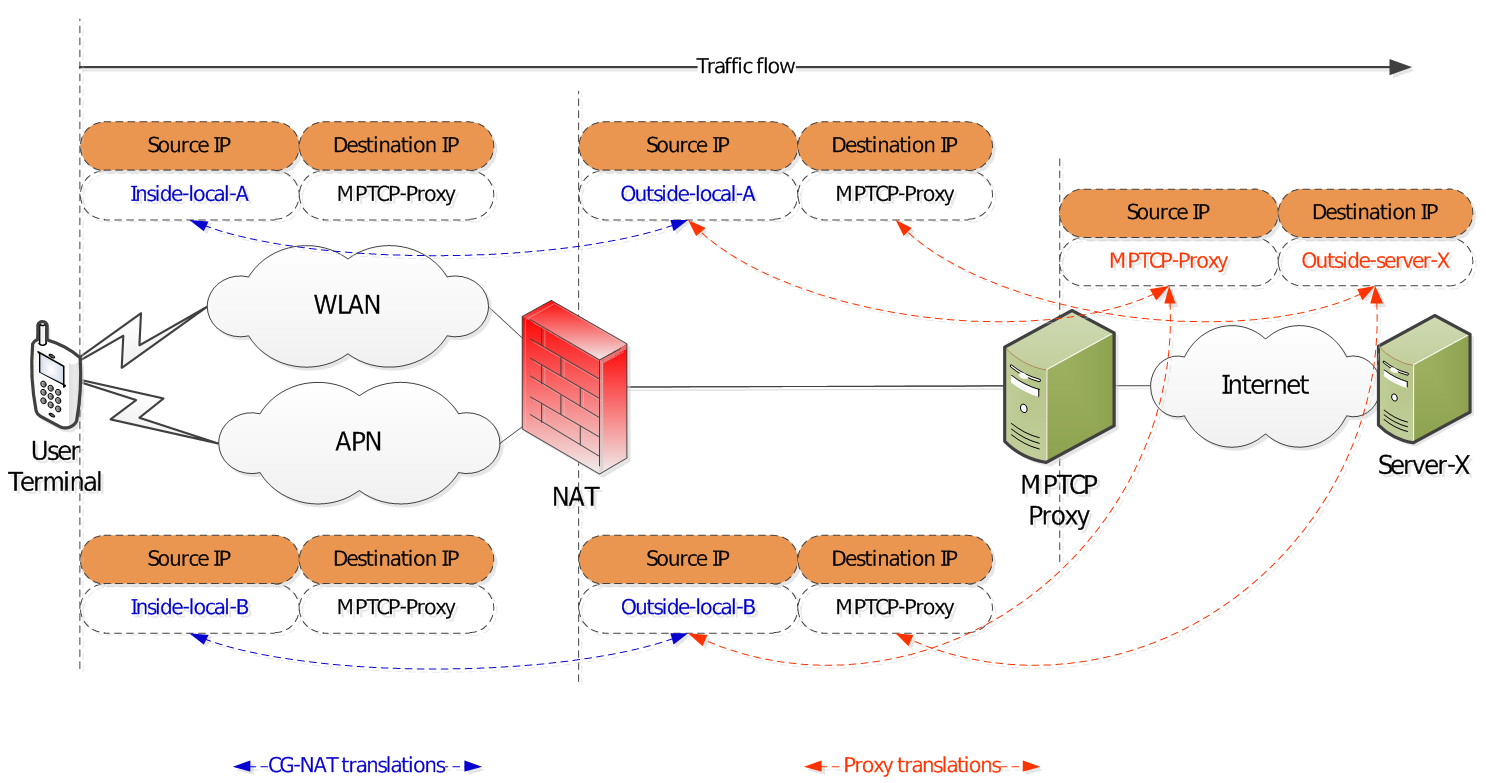
\includegraphics[scale=0.3]{figures/oro/oro_mptcp_nat.png}
	\caption{Pre-proxy NAT}
    	\label{fig:oro_mptcp_nat}
\end{figure}



{\em Cazul 1}: (figura \ref{fig:oro_mptcp_nat}) Pre-Proxy NAT – funcția NAT este plasata intre terminal si MPTCP Proxy.
\begin{itemize}
 \item	Proxy-ul trebuie să fie configurat cu o adresă IP publică sau cu un pool pentru a avea conectivitate directă la Internet.
\item Funcția NAT trebuie să fie dimensionat pentru dublul sesiunilor TCP.
\item Impactul NAT asupra funcției Proxy trebuie să fie considerat pentru o funcționare adecvată a Proxy-ului
\end{itemize}
 
  
{\em Cazul 2}: figura (\ref{fig:oro_mptcp_nat2}) Post-Proxy NAT - funcția NAT este plasata intre MPTCP Proxy si internet
\begin{itemize}
 \item	Proxy-ul poate folosi si adrese private.
\item	Există un avantaj față de cazul 1, deoarece numărul de fluxuri NAT este mai mic după Proxy, comparativ cu cazul anterior, din cauza lipsei fluxurilor MPTCP. De asemenea, protocolul MPTCP poate fi configurat cu o adresă IP publică, pentru a elimina complet necesitatea NAT pentru Proxy-ul MPTCP.
\item	Funcția NAT va rămâne în continuare pentru fluxurile de traficnon-TCP ale utilizatorilor.
 \end{itemize}
 
\begin{figure}[h]
	\centering
	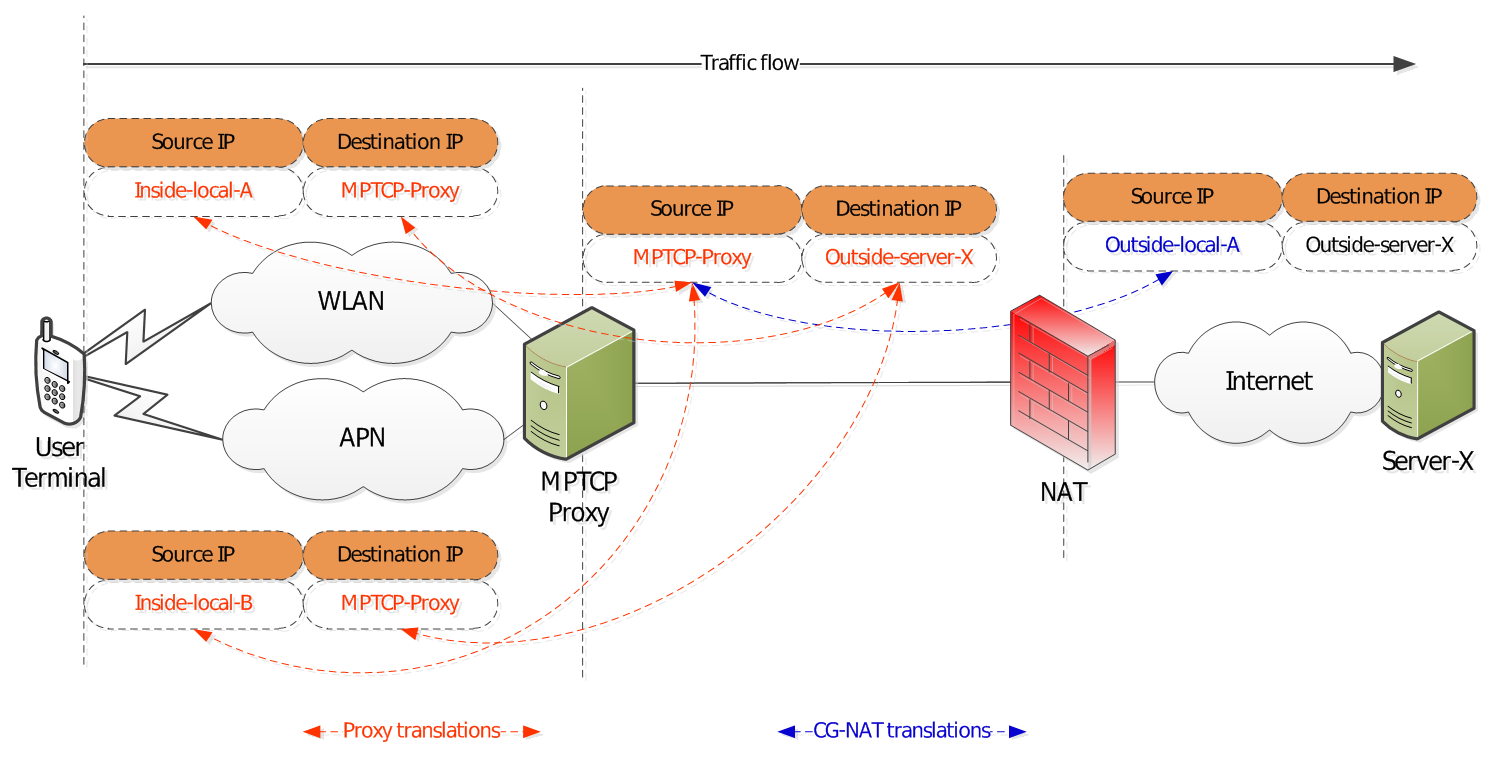
\includegraphics[scale=0.3]{figures/oro/oro_mptcp_nat2.png}
	\caption{Post-proxy NAT}
    	\label{fig:oro_mptcp_nat2}
\end{figure}


